\begin{center}
    \begin{figure}[H]
        \centering

        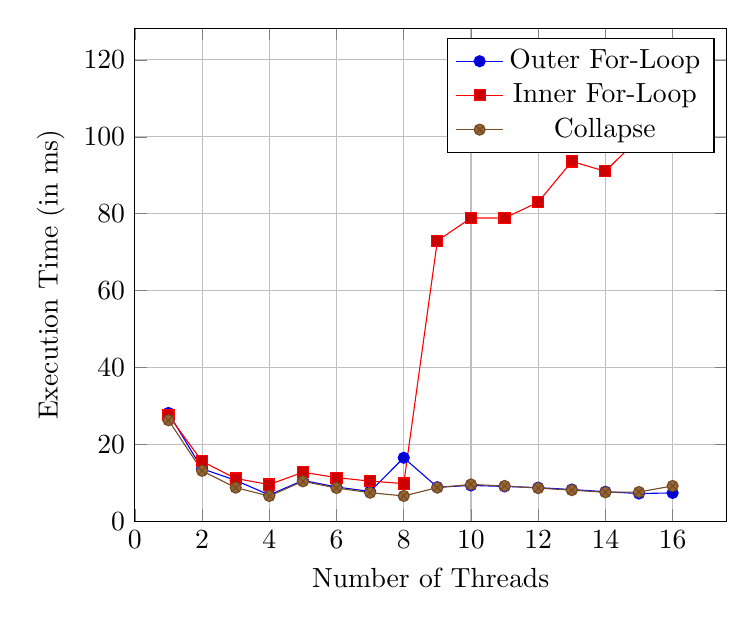
\begin{tikzpicture}
            \begin{axis}[
                title={},
                width=0.75\textwidth,
                xlabel={Number of Threads},
                ylabel={Execution Time (in ms)},
                xmin=0,
                ymin=0,
                grid=major
            ]
                \addplot coordinates {
                    (1,28.1787)(2,13.6684)(3,10.6587)(4,6.841)(5,10.6448)(6,8.9229)(7,7.7613)(8,16.5284)(9,8.8759)(10,9.3305)(11,9.0727)(12,8.75325)(13,8.265)(14,7.6939)(15,7.22555)(16,7.37725)
                };
                \addlegendentry{Outer For-Loop}

                \addplot coordinates {
                    (1,27.5487)(2,15.6059)(3,11.1323)(4,9.5563)(5,12.7669)(6,11.3685)(7,10.444)(8,9.8202)(9,72.9501)(10,78.8844)(11,78.8677)(12,82.9903)(13,93.5949)(14,91.0306)(15,99.7156)(16,116.585)
                };
                \addlegendentry{Inner For-Loop}       

                \addplot coordinates {
                    (1,26.2787)(2,13.1285)(3,8.74935)(4,6.5788)(5,10.3955)(6,8.6642)(7,7.436)(8,6.6008)(9,8.76145)(10,9.5894)(11,9.1864)(12,8.6334)(13,8.10475)(14,7.5467)(15,7.62205)(16,9.2002)
                };
                \addlegendentry{Collapse}
            \end{axis}
        \end{tikzpicture}
        \caption{Emboss Performance Tests dice.png}
    \end{figure}
\end{center}